\documentclass[12pt, letterpaper, landscape]{article}

% ==================================================
% PACKAGES
% ==================================================
\usepackage[margin=0.8in]{geometry}
\usepackage{xcolor}
\usepackage{pagecolor}
\usepackage{enumitem}
\usepackage{listings}
\usepackage{graphicx}
\usepackage{wrapfig}
\usepackage{caption}
\usepackage{amsmath}
\usepackage{eso-pic}

\setlength{\parindent}{0pt}
\setlength{\parskip}{0pt}

% ==================================================
% PAGE COLORS
% ==================================================
\definecolor{pagebg}{HTML}{000000}
\definecolor{textwhite}{HTML}{FFFFFF}

\pagecolor{pagebg}
\color{textwhite}

% ==================================================
% CODE COLORS
% ==================================================
\definecolor{codebg}{HTML}{181818}
\definecolor{codegreen}{HTML}{98C379}
\definecolor{codegray}{HTML}{808080}
\definecolor{codepurple}{HTML}{C678DD}
\definecolor{codeblue}{HTML}{61AFEF}
\definecolor{codewhite}{HTML}{ABB2BF}
\definecolor{codemagenta}{HTML}{E06C75}

% ==================================================
% CODE LISTING STYLE
% ==================================================
\lstdefinestyle{mystyle}{
    backgroundcolor=\color{codebg},
    basicstyle=\ttfamily\footnotesize\color{codewhite},
    commentstyle=\color{codegreen},
    keywordstyle=\color{codeblue},
    stringstyle=\color{codepurple},
    numberstyle=\tiny\color{codegray},
    numbers=left,
    numbersep=8pt,
    breaklines=true,
    breakatwhitespace=false,
    keepspaces=true,
    showspaces=false,
    showstringspaces=false,
    showtabs=false,
    tabsize=4,
    frame=single,
    rulecolor=\color{codegray},
    framerule=0.3pt,
    captionpos=b,
    xleftmargin=1.5em,
    framexleftmargin=1em,
    framesep=6pt,
    columns=fullflexible,
    upquote=true
}

\lstset{style=mystyle}

% ==================================================
% BULLET STYLE
% ==================================================
\setlist[itemize]{
    label=\textcolor{textwhite}{\textbullet},
    leftmargin=2em,
    itemsep=0.5em,
    topsep=0.5em
}

% ==================================================
% REUSABLE PAGE HEADING
% ==================================================
\newcommand{\newnotepage}[1]{
    \clearpage
    \noindent{\LARGE\bfseries #1}\par
    \vspace{0.5em}
    \noindent\rule{\textwidth}{0.5pt}
    \vspace{1em}
}

% ==================================================
% IMAGE HELPER
%
% Usage:
% \notegraphic{width}{path/to/image.png}
%
% If the image is missing, a placeholder is shown
% so the template can still compile.
% ==================================================
\newcommand{\notegraphic}[2]{%
    \IfFileExists{#2}{%
        \includegraphics[width=#1]{#2}%
    }{%
        \fcolorbox{codegray}{codebg}{%
            \parbox[c][3cm][c]{%
                \dimexpr#1-2\fboxsep-2\fboxrule\relax
            }{%
                \centering\color{textwhite}\small
                Image placeholder\\[0.5em]
                \texttt{\detokenize{#2}}%
            }%
        }%
    }%
}

% ==================================================
% DOCUMENT
% ==================================================
\begin{document}


% Title page goes here
\thispagestyle{empty}
\vspace*{\fill}
\thispagestyle{empty}
\thispagestyle{empty}
\AddToShipoutPictureBG*{%
    \AtPageLowerLeft{%
        \put(0,0){%
            \makebox(0,0)[lb]{%
                \color{black}%
                \rule{\paperwidth}{\paperheight}%
            }%
        }%
        \put(\LenToUnit{0.5\paperwidth},%
             \LenToUnit{0.5\paperheight}){%
            \makebox(0,0){%
                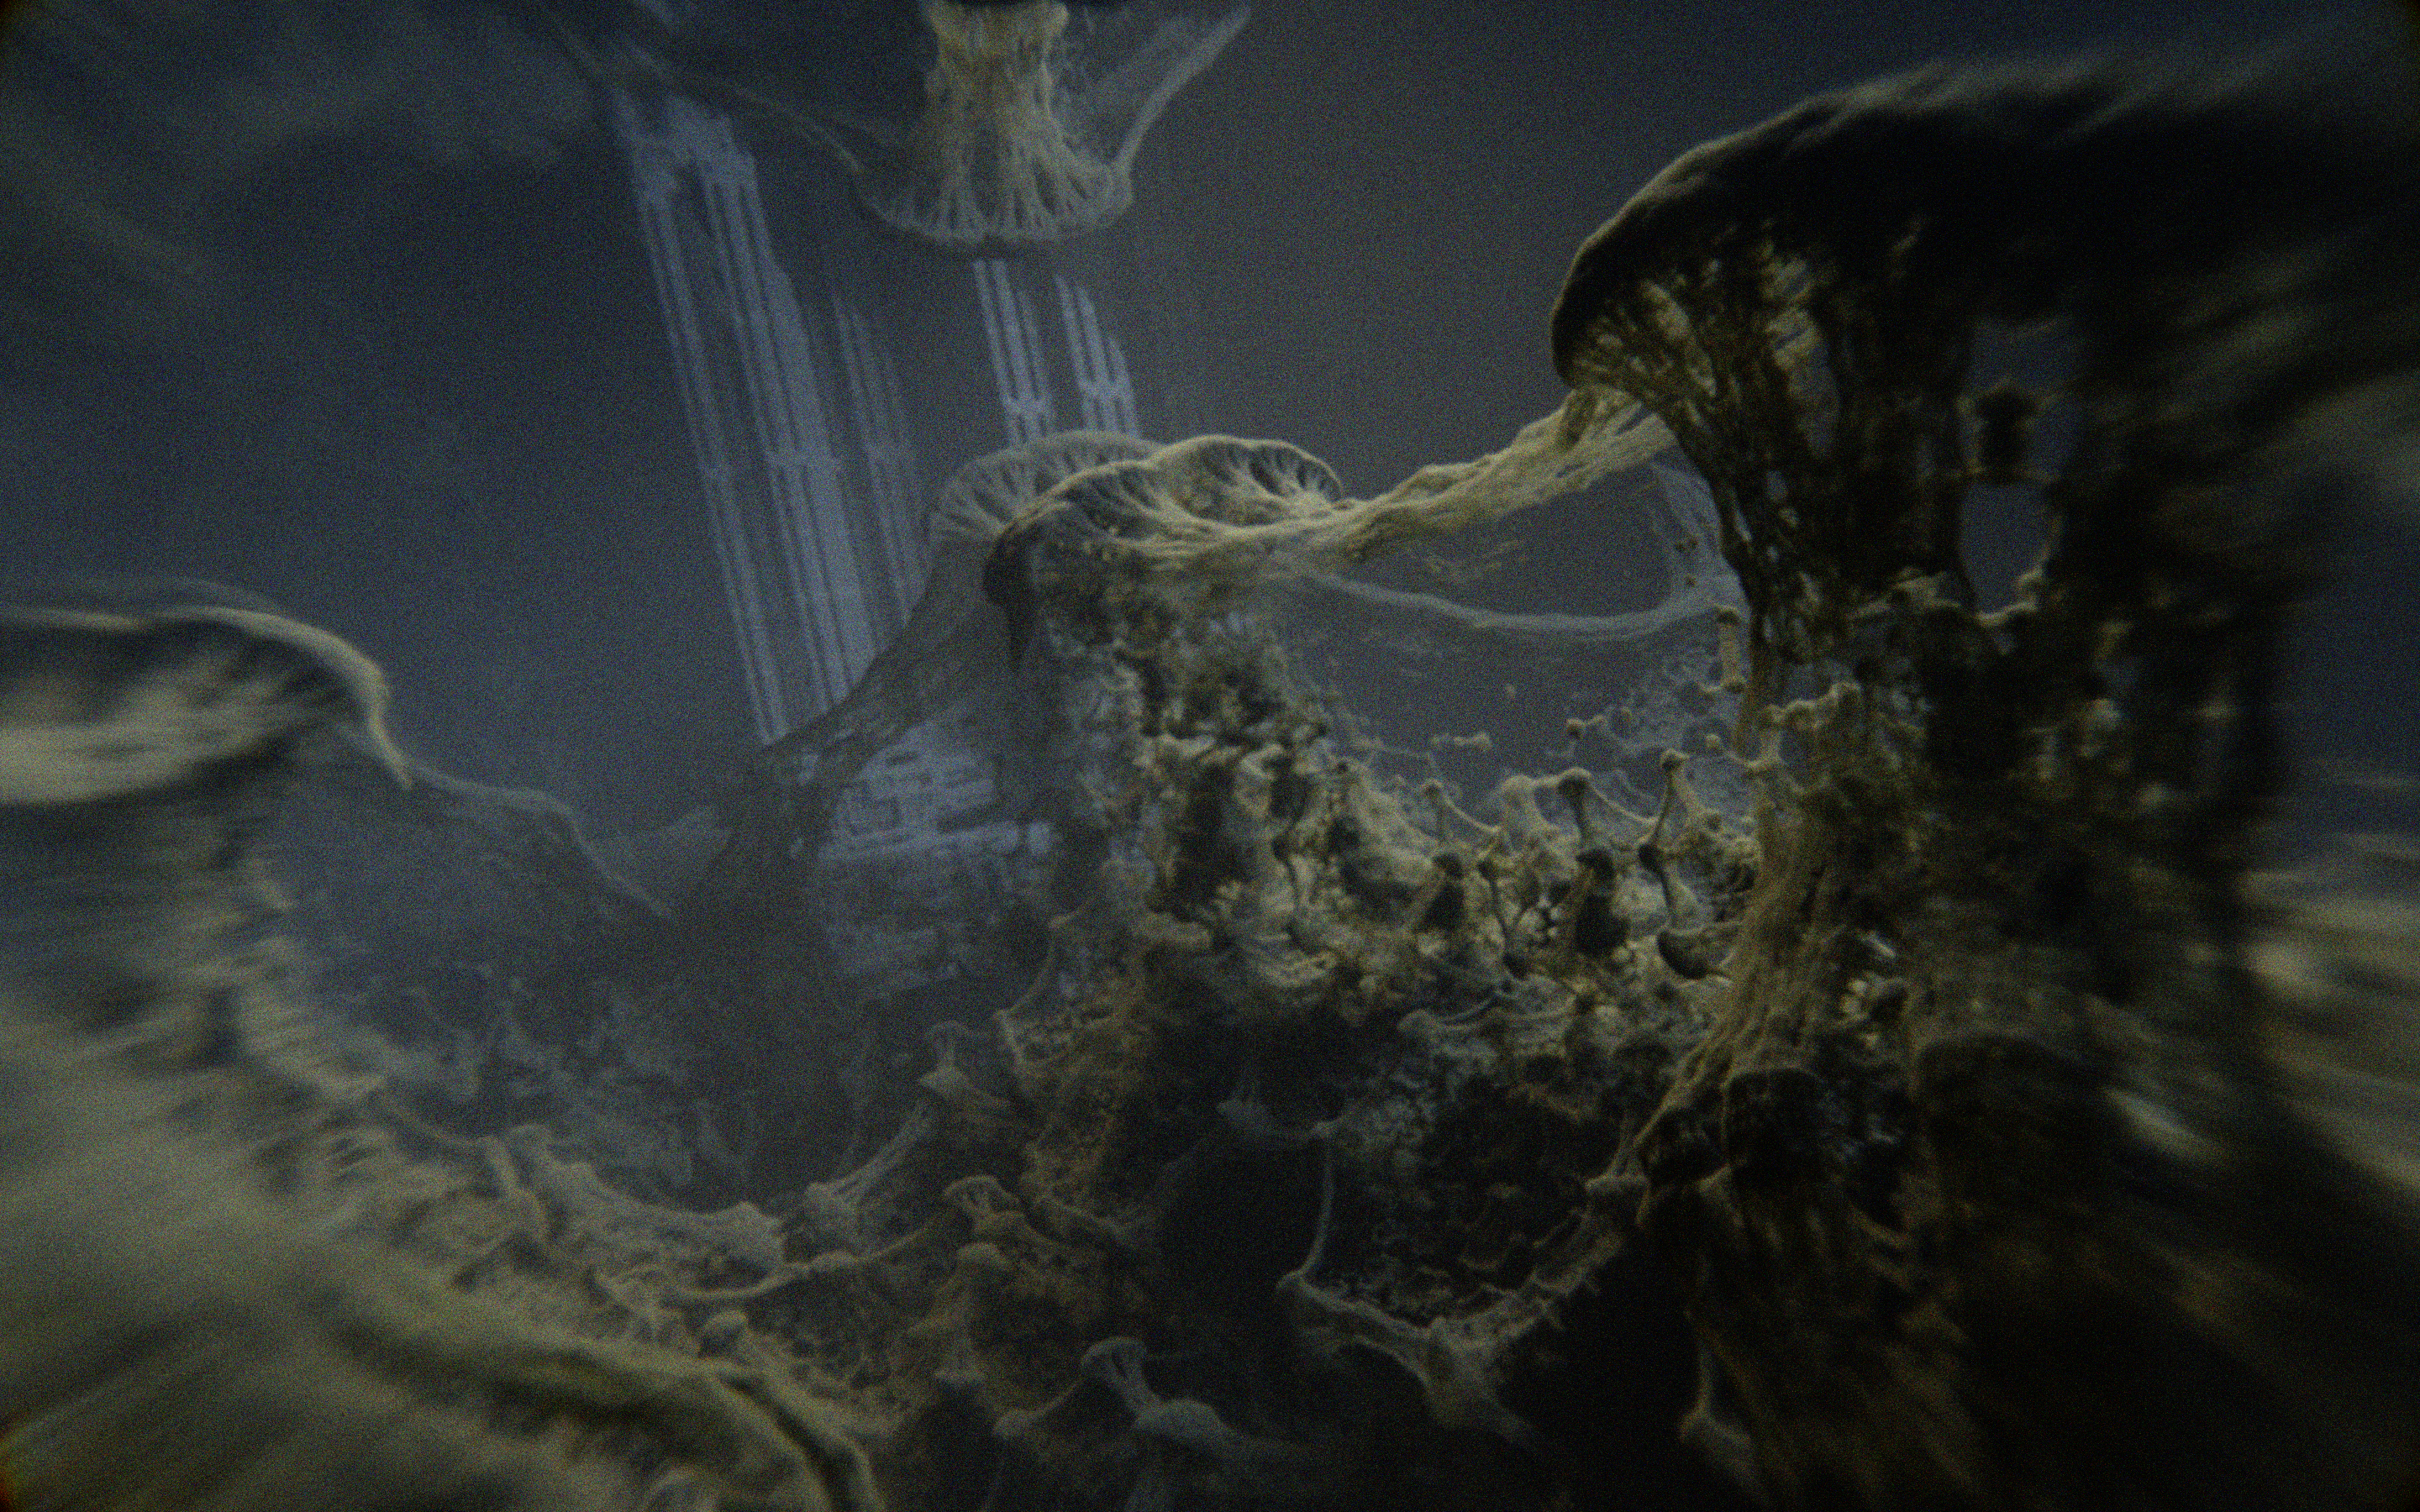
\includegraphics[
                    width=\paperwidth,
                    height=\paperheight,
                    keepaspectratio
                ]{test2.png}%
            }%
        }%
    }%
}
\vspace*{\fill}
\begin{center}
\color{textwhite}
\color{codeblue}
    \vspace{8cm}
    {\Huge\bfseries Implementing a Full Spectral Lens Sim\par}
    \vspace{1cm}
    {\large October 30, 2026\par}
    \vspace{1cm}
    {\Large Jon Baker (jb)\par}
    {\large twitter: @jbaker\_graphics, bsky: @jbakergraphics\par}
    {\large project blog: https://jbaker.graphics/}
\color{textwhite}
\end{center}
\vspace*{\fill}
\clearpage


% ==================================================
% PAGE 1: BASIC NOTES AND CODE
% ==================================================
\newnotepage{Snell's Law - Refraction}
\begin{wrapfigure}{r}{0.38\textwidth}
    \centering
    \notegraphic{0.36\textwidth}{lens/snell.png}
\end{wrapfigure}

\begin{itemize}
    \item {\large Refraction happens when we transition between media of different index of refraction (IoR), $N_{\text{1}}$ and $N_{\text{2}}$}
    \begin{itemize}
        \item {\large This is a unitless property of the material, and we are just taking a ratio of the two}
        \item {\large The ratio of these two properties is inverted, when you are going the other direction (air into glass vs glass into air)}
    \end{itemize}
    \item {\large We can calculate the result of the refraction in ray optics using the GLSL refract() function}
    \begin{itemize}
        \item {\large Parameters are the surface normal, the incident ray, and the ratio of $N_{\text{1}}$ and $N_{\text{2}}$, referred to as eta}
        \item {\large Result is the refracted ray, or a zero vector if the refraction math fails}
    \end{itemize}
\end{itemize}

\newnotepage{Snell's Law - Wave Interpretation}
\begin{wrapfigure}{r}{0.32\textwidth}
    \centering
    \notegraphic{0.3\textwidth}{lens/airtowater.png}
\end{wrapfigure}

\begin{itemize}
    \item {\large The IoR property actually describes the propagation speed of light in that medium, relative to how fast it travels in a vacuum}
    \item {\large This gives rise to another interpretation based on wave optics... pulses of incident energy arrive at some rate, and the bending ocurrs as a result, because they share phase at the boundary}
    \item {\large The specifics here are a little bit out of scope, but we can say that this is a phenomenon that changes with the rate of the pulses ariving at the interface}
    \begin{itemize}
        \item {\large "Rate" here refers to the frequency of the incident light - this property corresponds to its color, as it is proportionally related to the wavelength of the light by the constant speed of light C}
        \item {\large This variation of IoR with respect to frequency is referred to as "Dispersion", and it is a key concept in optical systems - it is the same phenomenon that is depicted on the cover of Dark Side of the Moon, and which gives rise to rainbows when it ocurrs inside of water droplets in the atmosphere}
    \end{itemize}
    \begin{figure}[htbp]
    \centering
    \notegraphic{0.5\textwidth}{lens/disperse.png}
    \end{figure}
\end{itemize}

\end{document}